\documentclass[journal,12pt,twocolumn]{IEEEtran}
\usepackage{setspace}
\usepackage{gensymb}
\usepackage{xcolor}
\usepackage{caption}
\singlespacing
\usepackage{siunitx}
\usepackage[cmex10]{amsmath}
\usepackage{mathtools}
\usepackage{hyperref}
\usepackage{amsthm}
\usepackage{mathrsfs}
\usepackage{txfonts}
\usepackage{stfloats}
\usepackage{cite}
\usepackage{cases}
\usepackage{subfig}
\usepackage{longtable}
\usepackage{multirow}
\usepackage{enumitem}
\usepackage{bm}
\usepackage{mathtools}
\usepackage{listings}
\usepackage{tikz}
\usetikzlibrary{shapes,arrows,positioning}
\usepackage{circuitikz}
\renewcommand{\vec}[1]{\boldsymbol{\mathbf{#1}}}
\DeclareMathOperator*{\Res}{Res}
\renewcommand\thesection{\arabic{section}}
\renewcommand\thesubsection{\thesection.\arabic{subsection}}
\renewcommand\thesubsubsection{\thesubsection.\arabic{subsubsection}}

\renewcommand\thesectiondis{\arabic{section}}
\renewcommand\thesubsectiondis{\thesectiondis.\arabic{subsection}}
\renewcommand\thesubsubsectiondis{\thesubsectiondis.\arabic{subsubsection}}
\hyphenation{op-tical net-works semi-conduc-tor}

\lstset{
language=Python,
frame=single, 
breaklines=true,
columns=fullflexible
}
\begin{document}
\theoremstyle{definition}
\newtheorem{theorem}{Theorem}[section]
\newtheorem{problem}{Problem}
\newtheorem{proposition}{Proposition}[section]
\newtheorem{lemma}{Lemma}[section]
\newtheorem{corollary}[theorem]{Corollary}
\newtheorem{example}{Example}[section]
\newtheorem{definition}{Definition}[section]
\newcommand{\BEQA}{\begin{eqnarray}}
        \newcommand{\EEQA}{\end{eqnarray}}
\newcommand{\define}{\stackrel{\triangle}{=}}
\newcommand{\myvec}[1]{\ensuremath{\begin{pmatrix}#1\end{pmatrix}}}
\newcommand{\mydet}[1]{\ensuremath{\begin{vmatrix}#1\end{vmatrix}}}
\bibliographystyle{IEEEtran}
\providecommand{\nCr}[2]{\,^{#1}C_{#2}} % nCr
\providecommand{\nPr}[2]{\,^{#1}P_{#2}} % nPr
\providecommand{\mbf}{\mathbf}
\providecommand{\pr}[1]{\ensuremath{\Pr\left(#1\right)}}
\providecommand{\qfunc}[1]{\ensuremath{Q\left(#1\right)}}
\providecommand{\sbrak}[1]{\ensuremath{{}\left[#1\right]}}
\providecommand{\lsbrak}[1]{\ensuremath{{}\left[#1\right.}}
\providecommand{\rsbrak}[1]{\ensuremath{{}\left.#1\right]}}
\providecommand{\brak}[1]{\ensuremath{\left(#1\right)}}
\providecommand{\lbrak}[1]{\ensuremath{\left(#1\right.}}
\providecommand{\rbrak}[1]{\ensuremath{\left.#1\right)}}
\providecommand{\cbrak}[1]{\ensuremath{\left\{#1\right\}}}
\providecommand{\lcbrak}[1]{\ensuremath{\left\{#1\right.}}
\providecommand{\rcbrak}[1]{\ensuremath{\left.#1\right\}}}
\theoremstyle{remark}
\newtheorem{rem}{Remark}
\newcommand{\sgn}{\mathop{\mathrm{sgn}}}
\newcommand{\rect}{\mathop{\mathrm{rect}}}
\newcommand{\sinc}{\mathop{\mathrm{sinc}}}
\providecommand{\abs}[1]{\left\vert#1\right\vert}
\providecommand{\res}[1]{\Res\displaylimits_{#1}}
\providecommand{\norm}[1]{\lVert#1\rVert}
\providecommand{\mtx}[1]{\mathbf{#1}}
\providecommand{\mean}[1]{E\left[ #1 \right]}
\providecommand{\fourier}{\overset{\mathcal{F}}{ \rightleftharpoons}}
\providecommand{\ztrans}{\overset{\mathcal{Z}}{ \rightleftharpoons}}
\providecommand{\system}[1]{\overset{\mathcal{#1}}{ \longleftrightarrow}}
\newcommand{\solution}{\noindent \textbf{Solution: }}
\providecommand{\dec}[2]{\ensuremath{\overset{#1}{\underset{#2}{\gtrless}}}}
\let\StandardTheFigure\thefigure
\def\putbox#1#2#3{\makebox[0in][l]{\makebox[#1][l]{}\raisebox{\baselineskip}[0in][0in]{\raisebox{#2}[0in][0in]{#3}}}}
\def\rightbox#1{\makebox[0in][r]{#1}}
\def\centbox#1{\makebox[0in]{#1}}
\def\topbox#1{\raisebox{-\baselineskip}[0in][0in]{#1}}
\def\midbox#1{\raisebox{-0.5\baselineskip}[0in][0in]{#1}}

\vspace{3cm}
\title{11.10.4.21}
\author{Lokesh Surana}
\maketitle
\section*{Class 11, Chapter 10, Exercise 4.21}

Q.21. Find equation of the line which is equidistant from parallel lines $9{x} + 6{y} - 7 = 0$ and $3{x} + 2{y} + 6 = 0$.

\solution Equation of lines are
\begin{align}
    {L}_1: \myvec{9&6}\vec{x} - 7 &= 0\\
    \implies {L}_1: \myvec{1&\frac{2}{3}}\vec{x} - \frac{7}{9} &= 0\\
    \implies \vec{n}_1 = \myvec{1\\\frac{2}{3}} \text{ and } {c}_1 &= \frac{7}{9}\\
    {L}_2: \myvec{3&2}\vec{x} + 6 &= 0\\
    \implies {L}_2: \myvec{1&\frac{2}{3}}\vec{x} + 2 &= 0\\
    \implies \vec{n}_2 = \myvec{1\\\frac{2}{3}} \text{ and } {c}_2 &= -2
\end{align}

The equation of desired line will be $\vec{n}^{\top}\vec{x} = c$.
As it is given that lines are parallel, $\vec{n}$ must be same as $\vec{n}_1$ and $\vec{n}_2$.
\begin{align}
	{L}: \myvec{1&\frac{2}{3}}\vec{x} - c = 0
\end{align}

The distance between two parallel lines $\vec{n}^{\top}\vec{x} = {c}_1$ and $\vec{n}^{\top}\vec{x} = {c}_2$ is given as
\begin{align}
	{d} &= \frac{\abs{{c}_1 - {c}_2}}{\norm{n}}
\end{align}

So for given lines, we need to solve
\begin{align}
	\frac{\abs{{c}_1 - {c}}}{\norm{n}} &= \frac{\abs{{c}-{c}_2}}{\norm{n}}\\
	\implies \frac{\abs{\frac{7}{9} - {c}}}{{\sqrt{1^2 + \brak{\frac{2}{3}}^2}}} &= \frac{\abs{{c} + 2}}{{\sqrt{1^2 + \brak{\frac{2}{3}}^2}}}
\end{align}

Case 1.
\begin{align}
	\frac{7}{9} - {c} &= -{c} + 2\\
    \implies -\frac{7}{9} &= 2\\
    \text{ (not possible) } 
\end{align}

Case 2.
\begin{align}
    \frac{7}{9} - {c} &= {c} + 2\\
    \implies 2{c} &= -\frac{11}{9}\\
    \implies {c} &= -\frac{11}{18}
\end{align}

The equation of line is
\begin{align}
    {L}: \myvec{1&\frac{2}{3}}\vec{x} - c &= 0\\
    {L}: \myvec{1&\frac{2}{3}}\vec{x} +  \frac{11}{18}&= 0\\
    \implies {L}: \myvec{18&12}\vec{x} + 11 &= 0\\
\end{align}

\begin{figure}[!htb]
    \centering
    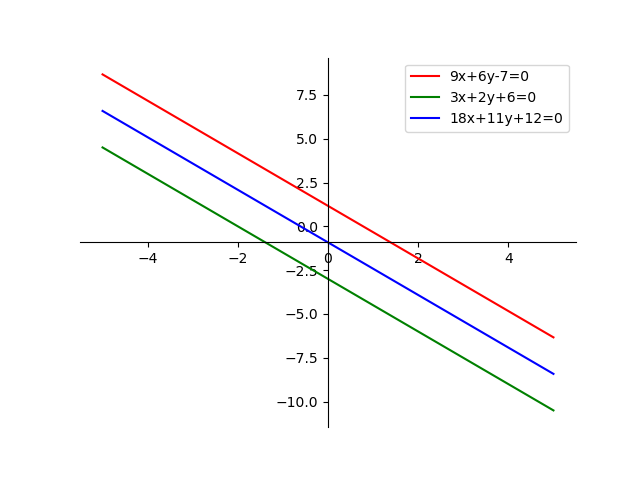
\includegraphics[width=\columnwidth]{figs/line.png}
    \caption{Given lines and equidistant line}
    \label{fig:line}
\end{figure}

\end{document}